\section{Теория}
	Генераторы случайных чисел разделяются на:
	\begin{itemize}
		\item аппаратные
		\item табличные
		\item алгоритмические
	\end{itemize}
	В данной лабораторной работе реализованы два последних из них
	
	\subsection{Алгоритмический генератор}
	Алгоритмический генератор использует одно или несколько значений для вычисления нового числа, после чего также используется для генерации последующих чисел.  
	
	В данной работе был использован линейный конгруэнтный метод. Последовательность в нём вычисляется по формуле
	\begin{equation}
		X_{n+1} = (aX_n + c)\;mod\;m,\,n \ge 1
	\end{equation}
	В данной лабораторной использованы значения из минимального стандартного генератора случайных чисел: $a = 16807$, $c = 2147483647$, $m = {MAX\_INT}$. 
	В качестве начального значения $X_1$ используется системное время.
	
	\subsection{Табличный генератор}
	Табличный генератор использует заранее подготовленные последовательности хранящиеся в памяти компьютера. 
	
	В лабораторной работе файлы были сгенерированы при помощи стандартной библиотеки языка $C\#$. Начальное значение генерируется так же и обозначает смещение относительно начала файла.
	
	\subsection{Критерий оценки}
	В качестве статистического критерия оценки случайности был выбран критерий "хи-квадрат". В первую очередь вычисляется статистика $V$
	\begin{equation}
		V = \frac{1}{n} \sum^{max}_{s=min}(\dfrac{Y^2_i}{p}) - n
	\end{equation}
	где $n$ - длина последовательности, $[min, max)$ - диапазон чисел, $Y_i$ - количество повторений числа $i$, $p=1/(max-min)$.
	
	После этого вычисляется критерий - квантиль хи-квадрат (степень свободы $max - min - 1$) от значения $V$. Полученное значение предлагается интерпретировать следующим образом:
	\begin{itemize}
		\item <0.1 или >0.9 - последовательность считается недостаточно случайной.
		\item >0.1 и <0.9 - последовательность считается случайной.
	\end{itemize}

\section{Работа программы}
	Для демонстрации работы критерия предоставленны 10 полей ввода. Оценка производятся для целых чисел от 0 до 9. Примеры работы программы приведены на рисунках \ref{pic:1}, \ref{pic:2} и \ref{pic:3}.
	
	\begin{figure}[h]
		\begin{center}
			{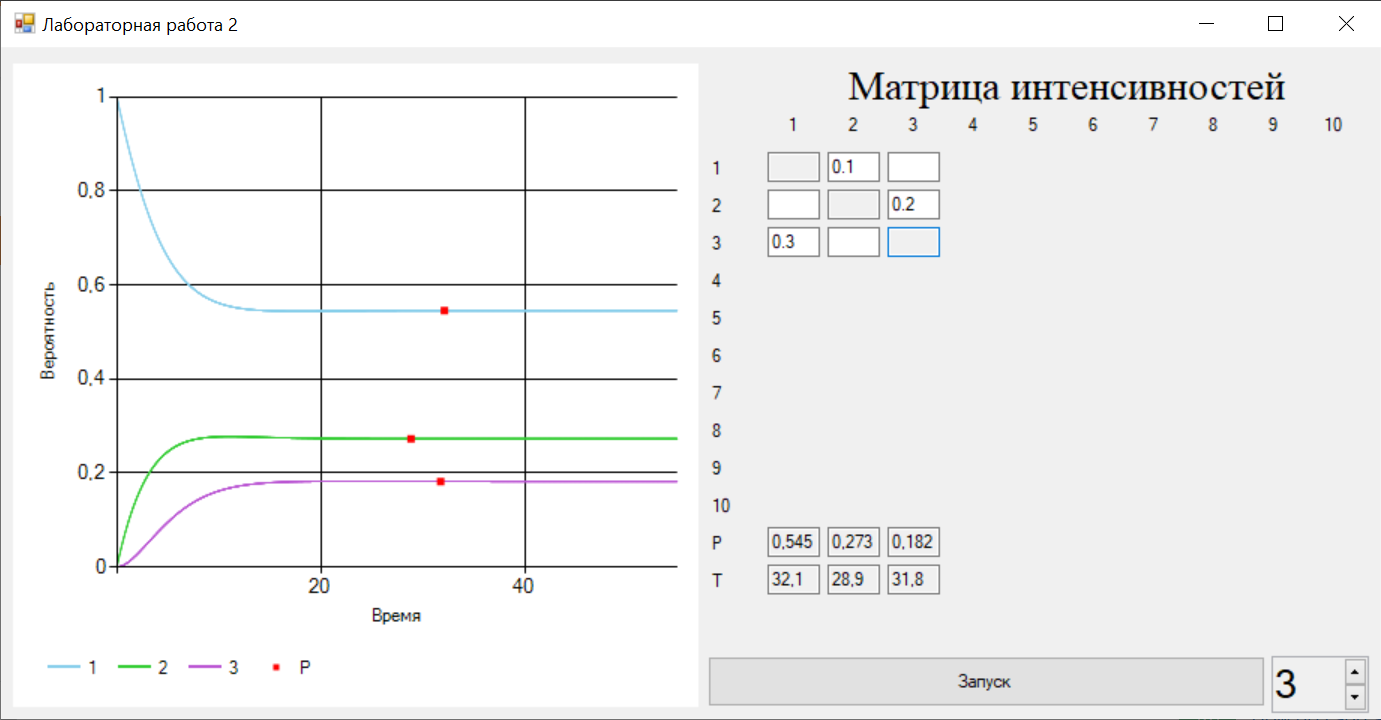
\includegraphics[scale=0.6]{1.png}
			\caption{Введена последовательность из одинаковых чисел}
			\label{pic:1}}
		\end{center}
	\end{figure}

	\begin{figure}[h]
		\begin{center}
			{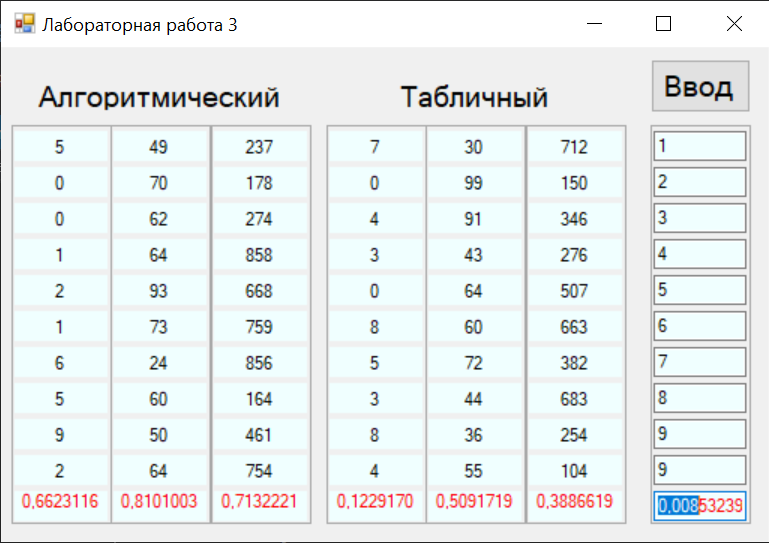
\includegraphics[scale=0.6]{2.png}
			\caption{Введена последовательность из разных чисел}
			\label{pic:2}}
		\end{center}
	\end{figure}
	
	\begin{figure}[h]
		\begin{center}
			{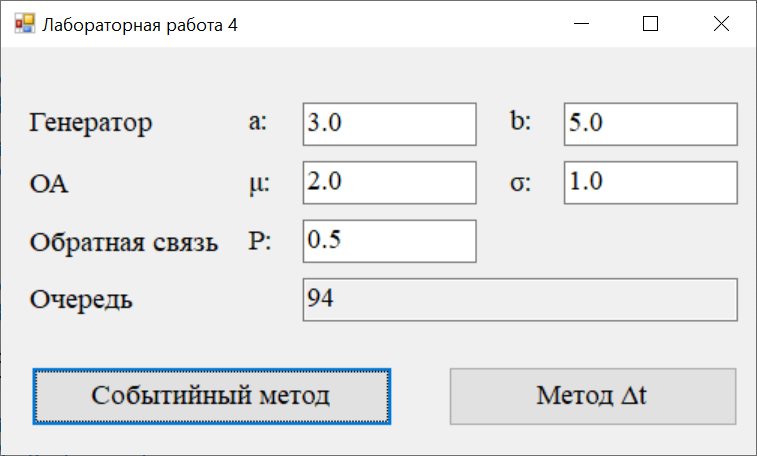
\includegraphics[scale=0.6]{3.png}
			\caption{Введена случайная последовательность}
			\label{pic:3}}
		\end{center}
	\end{figure}